\chapter{Experimental Design}

To test the effect of a barrier's height on the probability of tunneling, I used a combination of procedures and conventions from the experiments of John Bush, Yves Couder, and specifically, Eddi 2009 (CITE!). These elements were then slightly modified to fit some of the unique features of my experiment. In particular, I aim to give some of the reasoning behind the tray design and data collection techniques, both of which are not well described in the literature.

\section{Materials}
\subsection{Tray}
The tray was designed to guide the droplet to make a perpendicular collision with the barrier, but also to allow waves to decay. The tray is shown in \refFig{tray}. The rhombus shape serves to guide the droplet and the thin oil layer prevents too much interference from the walls. 

barrier height
black paint



\begin{figure}[h]
	\centering
	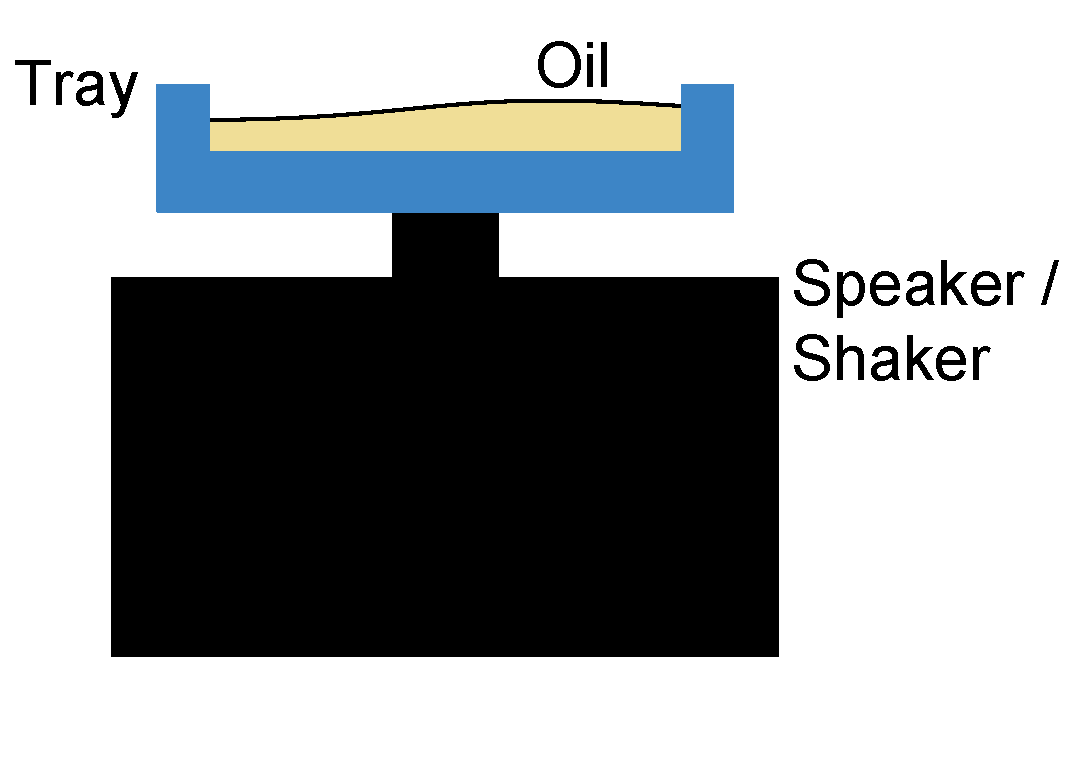
\includegraphics[scale=0.35]{HQASetup.pdf}
	\caption{The specifications of the tray design. }
	\label{tray}
\end{figure}

\subsection{Silicon Oil}
    The silicone oil used in this experiment had a viscocity of 20 cSt (the thickness is a little closer to water than olive oil) obtained from Clearco Products Co., Inc. (CAS No: 63148-62-9). The 20 cSt viscocity of Bush's group was chosen over the 50 cSt viscocity of Courder's group because ???. The tray could be filled with half a pint (?) of the fluid.
    
    It is of vital importance to keep the oil as clean as possible because it keeps the droplet floating for longer. This means protecting both from particulate matter that is already in the tray and from the particulate matter that might float on to the surface of the oil. The first problem was tackled by thoroughly cleaning the tray immediately before use. The second problem was mitigated in two steps: first, the experiment was done as soon as possible after the oil was initially poured into the tray; and second, a shield was placed over the tray to block dust.     

\subsection{Accelerometer}  
      

\subsection{Camera}    
 
\section{Setup}

\section{Data Collection}

